\documentclass[10pt,a4paper]{article}
\usepackage[utf8]{inputenc}
\usepackage[english]{babel}
\usepackage[T1]{fontenc}
\usepackage{amsmath}
\usepackage{amsfonts}
\usepackage{amssymb}
\usepackage{makeidx}
\usepackage{graphicx}
\usepackage{fourier}
\usepackage{color}
\usepackage{hyperref}
\usepackage[left=2cm,right=2cm,top=2cm,bottom=2cm]{geometry}
\author{Felipe Bruno, Vincent Noculak}
\title{Space Physics Project}

\begin{document}

\maketitle
\newpage
\tableofcontents
\newpage


\section{Introduction}

In this project we are going to study the space weather of the northern hemisphere of the earth at the 6. January 2011 between 18 and 24 o'clock universal time. We are going to do this by analysing the data of the ACE, SuperDARN, AMPERE, Ground-based magnetometers and All-Sky Cameras.

The phenomenons of space weather are mostly driven by the solar wind and its IMF (interplanetary magnetic field). The most important phenomenon of the interaction of the IMF and the terrestrial magnetic field is the Dungey cycle. This cycle can only happen when there is a southward IMF. It consists of the following steps which take approximately 12 hours to complete.

It begins with magnetic reconnection at the magnetopause between the in the opposite direction pointing magnetic field lines of the IMF and the earth. Due to the magnetic tension force and the solar wind, the reconnected field lines get dragged into the tail of the earth. The adding of magnetic flux to the tail compresses the plasma sheet. Now magnetic reconnection occurs in the tail. The reconnected and now again closed field lines of the earth return to the dayside where the cycle can begin anew.






\section{Instruments}

\subsection{All-Sky Camera}

In our project we are going to use the data of All-Sky cameras located in Svalbard at Ny Ålesund. These instruments are used to investigate the occurrence of auroras against time.
 Using a fish-eye lens, All-Sky cameras are able to take images of the whole sky. With an optical filter they can target the characteristic green and red light of the aurora. The cameras we are using have the filters at 5577 Å and 6300 Å. The cameras also include a photon counter to measure the brightness to the auroras. At \ref{a1} a typical diagram using an All-Sky Camera can be seen. While the colour gives the brightness, the x-axis gives the time and the y-axis gives the elevation. The diagram is made by taking the middle column of pixels in every photo the camera has taken and lining them up in the right time order.

\begin{figure}[h]
	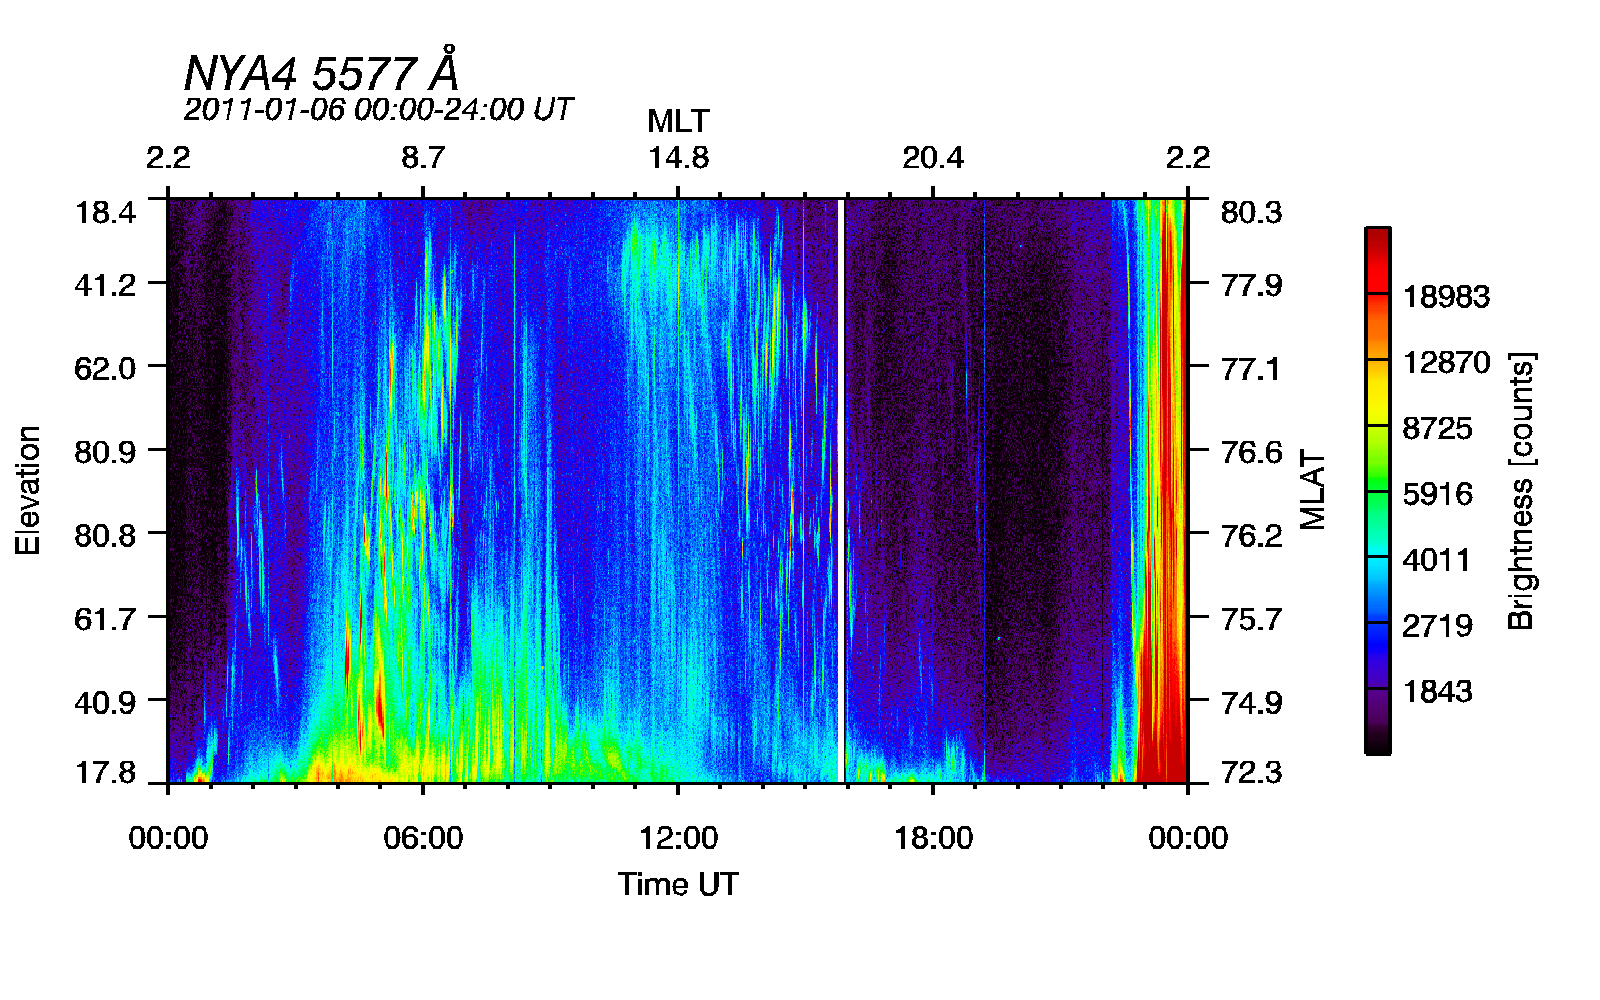
\includegraphics[scale = 0.25]{am_0024_5577.png}
	\centering
	\caption{Graphic of the All-Sky camera}
	\label{a1}
\end{figure}

\subsection{ACE}

The Advanced Composition Explorer, short ACE, is a satellite from NASA, which is among other things used to study the solar wind and its magnetic field. It orbits around the sun at the Lagrangian point $L_1$ so that it is always at a stable point between the earth and the sun, about $1.5 \cdot 10^6 km$ away from earth. 
One instrument of the satellite we are going to use is the SWEPAM (Solar Wind Electron, Proton and Alpha Monitor). With the instrument we can analysize the solar wind bulk speed to determine how much time it will need from the satellite to the earth. 
The other instrument we will use is the MAG (Magnetometer) to study the magnetic field of the solar wind.


\subsection{SuperDARN}

SuperDARN (Super Dual Auroral Radar Network) is a network of radars that consists of more than 30 low-power high frequency radars. It is used to measure plasma convection in the F-Region of the ionosphere at a high latitude. In \ref{s1} the area the radars of superDARN cover is shown. It can be seen that nearly the whole northern polar cap is covered by the radars. On Russia's side some ground at high latitude is not covered by the radars.
The radars are using the Doppler effect to measure convection. They send out electromagnetic waves at a specific frequency. In the Ionosphere the waves get reflected and have a Doppler shift due to movement of the plasma. From the change in frequency of the waves which return to the instruments, the velocity of the plasma can be determined.

\begin{figure}[h]
	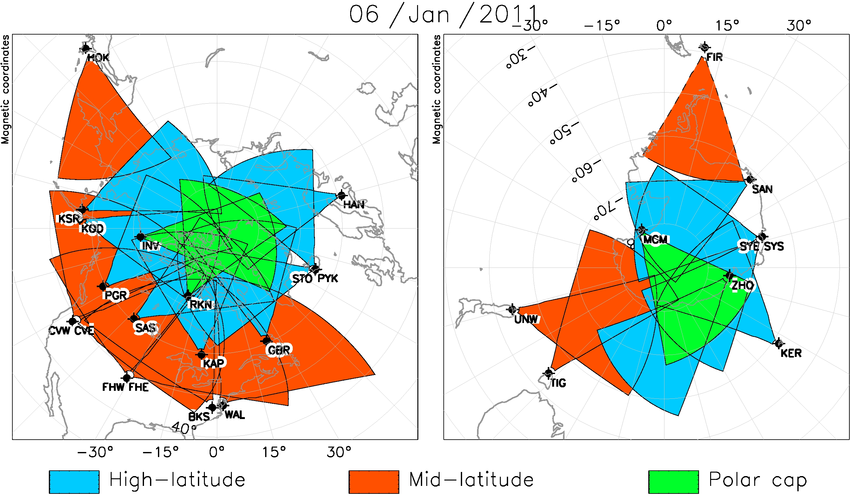
\includegraphics[scale = 1.5]{sd_1.png}
	\centering
	\caption{Covered area of the SuperDARN}
	\label{s1}
\end{figure}

\subsection{AMPERE}

AMPERE stands for "Active Magnetosphere and Planetary Electrodynamics Response Experiment". It uses the over 60  Iridium satellites which are orbiting earth to get information about the space weather. On the satellites are magnetometers to measure magnetic fields. From the measurement of those fields, field-aligned currents can be derived, using Amperes law. Thus the currents drawn in the diagrams belonging to AMPERE are not measured directly. Because of the amount of iridium satellites, the measurements are always covering the whole earth.

\subsection{Ground-based magnetometers}

In this project we are going to analyse the data on Ground-based magnetometers. Most of the magnetometers we are using are located in Norway, Sweden or Finland. A current always generates a magnetic field (Ampere's law). Hence by measuring the magnetic field on the ground, currents in the Ionosphere can be measured indirectly.




\section{Sources}

Websites:

	\url{http://tid.uio.no/plasma/aurora/tech.html}
	
	\url{https://en.wikipedia.org/wiki/Advanced_Composition_Explorer}
	
	\url{https://en.wikipedia.org/wiki/Super_Dual_Auroral_Radar_Network}
	
	\url{https://en.wikipedia.org/wiki/Iridium_satellite_constellation}
	
	\url{http://www.jhuapl.edu/newscenter/pressreleases/2010/100818.asp}
	
	\url{https://directory.eoportal.org/web/eoportal/satellite-missions/a/ampere}
	
Graphics:

	\url{http://tid.uio.no/plasma/aurora/data.php}
	
	\url{http://vt.superdarn.org/tiki-index.php?page=radarFoV}


\end{document}